
\section{\texorpdfstring{$\Phi^{\varGamma}$}{Phi-Gamma}的不变性：命题 11.2.8 的证明}
\label{sec:invariance-phi-gamma}

考虑把 $(H^{a},J^{a})$ 连接到 $(H^{b},J^{b})$ 的两个\trRegular\trHomotopy{} $\varGamma_{0}$ 与 $\varGamma_{1}$。我们要证明 $\Phi^{\varGamma_{0}}$ 与 $\Phi^{\varGamma_{1}}$ 在\trHomotopy{}的层面上相等。为此，我们要构造一个介于 $\Phi^{\varGamma_{0}}$ 与 $\Phi^{\varGamma_{1}}$ 之间的\trHomotopy
\[
S\colon CF_{\star}(H^{a},J^{a})\longrightarrow CF_{\star+1}(H^{b},J^{b})
\]
——换句话说，也就是一个满足关系式
\[
\Phi^{\varGamma_{1}}-\Phi^{\varGamma_{0}}
=S\circ\partial_{(H^{a},J^{a})}+\partial_{(H^{b},J^{b})}\circ S
\]
的 $S$（这就蕴含了所期望的等式）。

于是我们考虑一个“\trHomotopy{}的\trHomotopy” $\varGamma=(\varGamma_{\lambda})_{\lambda\in[0,1]}$，它把 $\varGamma_{0}$ 与 $\varGamma_{1}$ 连接起来，我们并且假定它在 $\lambda=0$ 与 $\lambda=1$ 的附近是\trStationary{}的。我们可以把它选得使存在一个 $R>0$，具有如下性质：对每个 $\lambda\in[0,1]$，
\[
\varGamma_{\lambda}(s)=
\begin{cases}
(H^{a},J^{a})\text{，} & s\le-R\text{，}\\
(H^{b},J^{b})\text{，} & s\ge R\text{。}
\end{cases}
\]
见\cref{fig:gamma-square}。我们要利用 $\scr{J}$ 的\trContractible{}性（更确切地说，是它\trSimplyConnected{}的这一事实）。

我们把 $\varGamma$ 视为一个映射 $(H,J)$，其中
\[
\begin{aligned}
H&\colon[0,1]\times\RR\times S^{1}\times W\longrightarrow\RR\text{，}\\
J&\colon[0,1]\times\RR\longrightarrow\operatorname{End}(TW)\text{，}
\end{aligned}
\]
并且对每个 $(\lambda,s)\in[0,1]\times\RR$ 都有 $J^{\lambda}_{s}\in\scr{J}$。我们可以——而且我们也确实如此——假定 $H$ 与 $J$ 都是 $\cC^{\infty}$ 类的。对每个 $\lambda\in[0,1]$，这些数据都定义了一个带参数的\trFloerEquation。利用这些方程，我们便或多或少地按照\cref{sec:morphism-phi-gamma}中的同一套方案来证明\cref{thm:homology-independent-gamma}。

\begin{figure}[htbp]
\centering
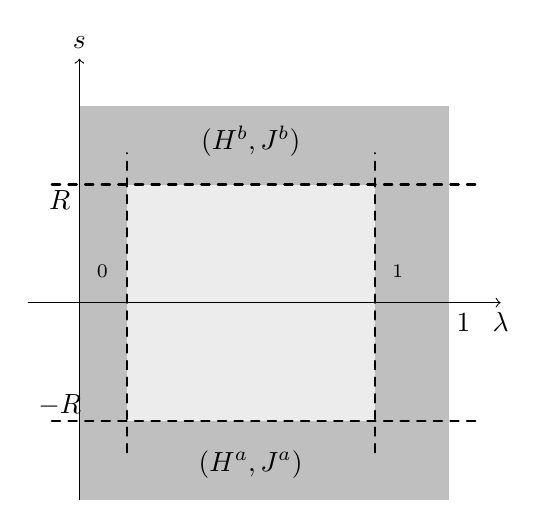
\begin{tikzpicture}[line cap=round,line join=round]
\fill[gray!50] (-0.6,-2.5) rectangle (4.1,2.5);
\fill[gray!15] (0,-1.5) rectangle (3.15,1.5);
\draw[dashed,thick] (0,-1.9) -- (0,1.9);
\draw[dashed,thick] (3.15,-1.9) -- (3.15,1.9);
\draw[dashed,thick] (-0.95,1.5) -- (4.45,1.5);
\draw[dashed,thick] (-0.95,-1.5) -- (4.45,-1.5);
\node at (1.575,2.05) {$(H^{b},J^{b})$};
\node at (1.575,-2.05) {$(H^{a},J^{a})$};
\node at (-0.3,0.4) {$\varGamma_{0}$};
\node at (1.575,0.4) {$\varGamma$};
\node at (3.45,0.4) {$\varGamma_{1}$};
\draw[->] (-0.6,-2.5) -- (-0.6,3.1) node[above] {$s$};
\draw[->] (-1.25,0) -- (4.75,0) node[below] {$\lambda$};
\node at (-0.85,1.30) {$R$};
\node at (-0.85,-1.30) {$-R$};
\node at (4.28,-0.25) {$1$};
\end{tikzpicture}
\caption{}
\label{fig:gamma-square}
\end{figure}

\subsection{\trFloerEquation}
\label{subsec:floer-equations}

取定一个 $\lambda\in[0,1]$，对 $\varGamma_{\lambda}(s)=(H^{\lambda}_{s,t},J^{\lambda}_{s})$ 考虑方程
\[
\frac{\partial u}{\partial s}+J^{\lambda}_{s}(u)\frac{\partial u}{\partial t}
+\operatorname{grad}_{u}H^{\lambda}_{s,t}=0
\]
与它相应的解空间
\[
\scr{M}^{\varGamma_{\lambda}}
=\bigl\{u\colon\RR\times S^{1}\longrightarrow W
\ \bigm|\ u\ \text{\trContractible{}，且}\ E(u)<+\infty\bigr\}\text{。}
\]
由\cref{thm:gamma-limits-critical-points}，我们知道
\[
\scr{M}^{\varGamma_{\lambda}}
=\bigcup_{\substack{x\in\operatorname{Crit}\scr{A}_{H^{a}}\\ y\in\operatorname{Crit}\scr{A}_{H^{b}}}}
\scr{M}^{\varGamma_{\lambda}}(x,y)\text{。}
\]
对 $x\in\operatorname{Crit}\scr{A}_{H^{a}}$ 与 $y\in\operatorname{Crit}\scr{A}_{H^{b}}$，\footnote{译注：原书将此下标多处印作 $\scr{A}_{H_{b}}$（$b$ 为 $H$ 的下标；本节内计九处——p.414 两处、p.419 一处、p.423 计算中六处）；按本章通例（如\cref{thm:transversality-gamma-h}中）均应作 $\scr{A}_{H^{b}}$（$b$ 为 $H$ 的上标），疑为排印之误，九处径改。——译者注}我们定义空间
\[
\scr{M}^{\varGamma}(x,y)=\bigl\{(\lambda,u)\ \bigm|\ \lambda\in[0,1],\ u\in\scr{M}^{\varGamma_{\lambda}}(x,y)\bigr\}\text{。}
\]

\begin{remark}\label{thm:cobordism-m-gamma}
我们可以把 $\scr{M}^{\varGamma}(x,y)$ 视为介于 $\scr{M}^{\varGamma_{0}}(x,y)$ 与 $\scr{M}^{\varGamma_{1}}(x,y)$ 这两个\trManifold{}之间的一个\trCobordism。事实上，如果
\[
\pi\colon\scr{M}^{\varGamma}(x,y)\longrightarrow[0,1]
\]
表示（到诸 $\lambda$ 的空间上的）投影，那么我们有
\[
\pi^{-1}(\lambda)=\scr{M}^{\varGamma_{\lambda}}(x,y)\text{。}
\]
我们还需要证明 $\scr{M}^{\varGamma}(x,y)$ 是一个\trManifold；这件事我们将在下一小节中做。
\end{remark}

\subsection{\trTransversality}
\label{subsec:transversality-gamma-lambda}%

我们将使用由形如
\[
h\colon[0,1]\times\RR\times S^{1}\times W\longrightarrow\RR
\]
的映射所组成的（\trPerturbation{}）空间 $\cC^{\infty}_{\varepsilon}$，其中的映射在 $\,]0,1[\,\times\RR\times W$ 中有\trCompact{}\trSupport{}，并且满足 $\|h\|_{\varepsilon}<+\infty$。令
\[
h^{\lambda}_{s,t}(z)=h(\lambda,s,t,z)\text{，}
\]
并令 $\varGamma=(H,J)$。我们有下面这个结果。

\begin{theorem}\label{thm:transversality-gamma-h}
在 $\cC^{\infty}_{\varepsilon}$ 中存在 $0$ 的一个邻域，以及此邻域内诸\trDense\trOpen{}子集的一个可数交 $\scr{H}_{\mathrm{reg}}$，使得若 $h\in\scr{H}_{\mathrm{reg}}$，则对 $\varGamma(h)=(H+h,J)$ 以及每个 $x\in\operatorname{Crit}\scr{A}_{H^{a}}$ 与每个 $y\in\operatorname{Crit}\scr{A}_{H^{b}}$，空间 $\scr{M}^{\varGamma(h)}(x,y)$ 都是一个维数为 $\mu(x)-\mu(y)+1$ 的\trManifoldWithBoundary，并且它的边界为
\[
\partial\scr{M}^{\varGamma(h)}(x,y)
=\bigl(\{0\}\times\scr{M}^{\varGamma_{0}}(x,y)\bigr)
\cup\bigl(\{1\}\times\scr{M}^{\varGamma_{1}}(x,y)\bigr)\text{。}
\]
\end{theorem}

在这条陈述中，我们使用的是 $\scr{M}^{\varGamma(h)}(x,y)$ 上由 $\RR\times\cC^{\infty}_{\mathrm{loc}}(\RR\times S^{1};W)$ 的\trTopology{}所诱导的\trTopology。

让我们先来看看在边界的附近会发生什么。设 $x\in\operatorname{Crit}\scr{A}_{H^{a}}$，并设 $y\in\operatorname{Crit}\scr{A}_{H^{b}}$。对一个取定的、任意的 $h\in\cC^{\infty}_{\varepsilon}$，我们来分析 $\scr{M}^{\varGamma(h)}(x,y)$ 在它的那些满足 $\lambda\in\{0,1\}$ 的点 $(\lambda,u)$ 附近的结构。

设 $\delta>0$ 充分小，使得
\[
\operatorname{Supp}(h)\subset[\delta,1-\delta]\times\RR\times S^{1}\times W
\]
并且使\textbf{\trIsotopy}（isotopy） $\varGamma=(H,J)$ 在 $\lambda\le\delta$ 时以及在 $\lambda\ge1-\delta$ 时都\trStationary。于是我们有：$\varGamma(h)=\varGamma_{0}$（若 $\lambda\le\delta$），$\varGamma(h)=\varGamma_{1}$（若 $\lambda\ge1-\delta$）。这样一来，显然
\[
\scr{M}^{\varGamma(h)}(x,y)\cap\{\lambda<\delta\}
=[0,\delta[\,\times\,\scr{M}^{\varGamma_{0}}(x,y)
\]
而且
\[
\scr{M}^{\varGamma(h)}(x,y)\cap\{\lambda>1-\delta\}
=\,]1-\delta,1]\,\times\,\scr{M}^{\varGamma_{1}}(x,y)\text{。}
\]
这就表明：在
\[
\{0\}\times\scr{M}^{\varGamma_{0}}(x,y)\cup\{1\}\times\scr{M}^{\varGamma_{1}}(x,y)
\]
的各点的邻域内，空间 $\scr{M}^{\varGamma(h)}$ 就具有定理所说的那种\trManifoldWithBoundary{}的结构。

接下来，我们遵循与第~8~章相同的方案（参见\cref{sec:results}末尾的概观）。我们的出发点是\cref{thm:floer-map-fredholm}的一个类似物，也就是\cref{thm:fgamma-fredholm}的一个、对 $[0,1]$ 中取定的 $\lambda$ 关于诸\trHomotopy{} $\varGamma_{\lambda}$ 成立的版本，其证明亦同。

\begin{theorem}\label{thm:fredholm-gamma-lambda}
对每个取定的 $\lambda\in[0,1]$、一切\trCriticalPoint{} $x\in\operatorname{Crit}\scr{A}_{H^{a}}$、$y\in\operatorname{Crit}\scr{A}_{H^{b}}$ 以及每个 $u\in\scr{M}^{\varGamma_{\lambda}}(x,y)$，算子 $(d\scr{F}^{\varGamma_{\lambda}})_{u}$ 都是一个\trIndex{}为 $\mu(x)-\mu(y)$ 的\trFredholmOperator。
\end{theorem}

利用这条定理，我们可以建立一个与\cref{thm:z-banach-manifold}相类似的陈述。为此，我们取定 $J=(J^{\lambda})_{\lambda\in[0,1]}$，并且如同\cref{sec:transversality}中那样，考虑\trFiberBundle
\[
\scr{E}\longrightarrow\scr{P}^{1,p}(x,y)\times\cC^{\infty}_{\varepsilon}\text{，}
\]
其中
\[
\scr{E}=\bigl\{(u,h,Y)\ \bigm|\ (u,h)\in\scr{P}^{1,p}(x,y)\times\cC^{\infty}_{\varepsilon},\
Y\in L^{p}(u^{\star}TW)\bigr\}\text{。}
\]
我们通过令
\[
\sigma_{\lambda}(u,h)=\frac{\partial u}{\partial s}+J^{\lambda}(u)\frac{\partial u}{\partial t}
+\operatorname{grad}_{u}(H^{\lambda}+h^{\lambda})
\]
来定义一族\trSection{} $(\sigma_{\lambda})_{\lambda\in[0,1]}$。正如在\cref{sec:morphism-phi-gamma}中那样（利用\cref{thm:phi-surjective-right-inverse}的那个类似物），我们可以证明：对每个 $\lambda\in[0,1]$，映射 $\sigma_{\lambda}$ 都\trTransverse{}于上面定义的\trFiberBundle{} $\scr{E}$ 的\trZeroSection。由此推出：同样的性质对 $\cC^{\infty}$ 映射
\[
\begin{aligned}
\sigma\colon\,]0,1[\,\times\,\scr{P}^{1,p}(x,y)\times\cC^{\infty}_{\varepsilon}
&\longrightarrow\scr{E}\\
(\lambda,u,h)&\longmapsto\sigma_{\lambda}(u,h)
\end{aligned}
\]
也成立，而这按\trImplicitFunctionTheorem{}便蕴含了\cref{thm:z-banach-manifold}的那个类似物。

\begin{proposition}\label{thm:z-gamma-banach}
设 $x\in\operatorname{Crit}\scr{A}_{H^{a}}$ 与 $y\in\operatorname{Crit}\scr{A}_{H^{b}}$，则定义为
\[
\bigl\{(\lambda,u,H+h)\ \bigm|\ \lambda\in\,]0,1[,\ h\in\cC^{\infty}_{\varepsilon},\
u\in\scr{M}^{\varGamma_{\lambda}}(x,y,(H+h)^{\lambda},J^{\lambda})\bigr\}
\]
的空间 $\scr{Z}(x,y,J)$ 是一个\trBanachManifold。
\end{proposition}

参数 $\lambda$ 的出现迫使我们（相对于\cref{subsec:tangent-space-z}）修改 $\scr{Z}(x,y,J)$ 在一点 $(\lambda,u,H+h_{0})$ 处的\trTangentSpace{}的表达式。在我们的新框架下，这个作为 $(d\sigma)_{(\lambda,u,H+h_{0})}$ 之\trKernel{}的空间，由一切满足方程\footnote{译注：原书诸处对 $\lambda$ 求导所得的参数方向场均作 $\frac{\partial J^{\lambda}}{\partial\lambda}\,\frac{\partial u}{\partial t}+\operatorname{grad}^{J^{\lambda}}\frac{\partial H}{\partial\lambda}$ 之形——本注所涉共四处：本节的\trTangentSpace{}方程与\trVectorField{} $V$（原书 p.417 两处）、下节 $L_{\rho}^{\varGamma}(a,0)$ 的展开式（p.428）与 $\widetilde{V}_{\rho_{n}}(\lambda,0)$ 的定义式（p.437）。按本书约定（第~5~章）$\operatorname{grad}^{J}H=-JX_{H}$，而 $J$ 亦随 $\lambda$ 变动，故\trGradient{}项对 $\lambda$ 求导应产生 $-\frac{\partial J^{\lambda}}{\partial\lambda}X$ 一项，即参数方向场应为 $\frac{\partial J^{\lambda}}{\partial\lambda}\Bigl(\frac{\partial u}{\partial t}-X\Bigr)+\operatorname{grad}^{J^{\lambda}}\frac{\partial H}{\partial\lambda}$（各处 $X$ 的下标随该处\trHamiltonian{}量而定），原书疑漏 $-\frac{\partial J^{\lambda}}{\partial\lambda}X$ 项；末处更把标量 $\frac{\partial H}{\partial\lambda}$ 直接加于\trVectorField，疑应为其\trGradient。四处径改。——译者注}
\[
a\frac{\partial J^{\lambda}}{\partial\lambda}(u)\Bigl(\frac{\partial u}{\partial t}-X_{(H+h_{0})^{\lambda}}(u)\Bigr)
+a\,\operatorname{grad}_{u}\frac{\partial(H+h_{0})^{\lambda}}{\partial\lambda}
+(d\scr{F}^{\varGamma_{\lambda}})_{u}(Y)+\operatorname{grad}_{u}(h^{\lambda})=0
\]
的 $(a,Y,h)\in\RR\times W^{1,p}\times\cC^{\infty}_{\varepsilon}$ 所组成。

为了证明\cref{thm:transversality-gamma-h}\footnote{译注：原书此处印作“定理 11.3.3”；按上下文，命题 11.3.5 的用途是收束定理 11.3.2 的证明（见下文“……我们推知 $\scr{M}^{\varGamma(h)}(x,y)$ 是一个\trManifoldWithBoundary”云云），而命题 11.3.5 的证明反而以定理 11.3.3 为依据，疑应为“定理 11.3.2”，此处径改。——译者注}，我们要使用下面这个结果。

\begin{proposition}\label{thm:pi-regular-values}
设 $\pi\colon\scr{Z}(x,y,J)\to\cC^{\infty}_{\varepsilon}$ 是投影。$\pi$ 在 $\cC^{\infty}_{\varepsilon}$ 中 $0$ 的一个邻域内的\trRegularValue{}所成之集，是这个邻域的一个\trDense\trOpen{}子集。\footnote{译注：这一陈述超出了\trSard--\trSmale{}定理之所予：该定理（\cref{thm:sard-smale}）只断言\trFredholm{}映射的\trRegularValue{}之集是诸\trDense\trOpen{}子集的一个可数交（残余集），既不断言它是“$0$ 的一个邻域内的\trDense\trOpen{}子集”（残余集虽然处处\trDense，但“$0$ 的邻域”无从由该定理得到，其本身一般不是任何一点的邻域），也不给出\trOpen{}性；\trOpen{}性须另行证明，且其论证要依赖诸解的\trEnergy{}一致界（如\cref{thm:energy-bound-compact}）。下文“设 $\scr{H}_{\mathrm{reg}}\subset\cC^{\infty}_{\varepsilon}$ 表示由这条命题所给出的那个邻域”沿用了同一说法。本处照原书排印，存疑备案（口径同第~8~章 §8.5 末关于 $\scr{H}_{\mathrm{reg}}$ 的注记）。——译者注}
\end{proposition}

\begin{proof}
这条陈述是\trSard--\trSmale{}定理（\cref{thm:sard-smale}）的一个直接应用，只要我们先证明 $\pi$ 是一个\trFredholm{}映射。为此，让我们证明：对每个 $(\lambda,u,H+h_{0})\in\scr{Z}(x,y,J)$，算子
\[
(d\pi)_{(\lambda,u,H+h_{0})}\colon
T_{(\lambda,u,H+h_{0})}\scr{Z}(x,y,J)\longrightarrow T_{h_{0}}\cC^{\infty}_{\varepsilon}
\]
——它具有 $(a,Y,h)\mapsto h$ 的形状——是一个\trFredholmOperator。设 $V$ 表示\trVectorField
\[
V=\frac{\partial J^{\lambda}}{\partial\lambda}(u)\Bigl(\frac{\partial u}{\partial t}-X_{H^{\lambda}+h_{0}^{\lambda}}(u)\Bigr)
+\operatorname{grad}_{u}\frac{\partial(H^{\lambda}+h_{0}^{\lambda})}{\partial\lambda}
\in L^{p}(u^{\star}TW)\text{。}
\]
按 $\scr{Z}(x,y,J)$ 的\trTangentSpace{}的表达式，我们看到 $(d\pi)_{(\lambda,u,H+h_{0})}$ 的\trKernel{}是空间
\[
\bigl\{(a,Y,0)\ \bigm|\ (a,Y)\in\RR\times W^{1,p}(u^{\star}TW)
\ \text{且}\ aV+(d\scr{F}^{\varGamma_{\lambda}})_{u}(Y)=0\bigr\}\text{。}
\]
于是让我们证明这个空间是有限维的。我们区分两种情形：
\begin{enumerate}[label=(\arabic*)]
\item $V\notin\operatorname{Im}\bigl((d\scr{F}^{\varGamma_{\lambda}})_{u}\bigr)$。在这种情形下，我们得到
\[
\operatorname{Ker}(d\pi)_{(\lambda,u,H+h_{0})}
=\bigl\{(0,Y,0)\ \bigm|\ Y\in\operatorname{Ker}(d\scr{F}^{\varGamma_{\lambda}}_{u})\bigr\}\text{，}
\]
它按\cref{thm:fredholm-gamma-lambda}是有限维的。
\item $V\in\operatorname{Im}\bigl((d\scr{F}^{\varGamma_{\lambda}})_{u}\bigr)$。我们选取一个 $Y_{0}\in W^{1,p}(u^{\star}TW)$，使得 $(d\scr{F}^{\varGamma_{\lambda}})_{u}(Y_{0})=V$。由此推出
\[
\operatorname{Ker}(d\pi)_{(\lambda,u,H+h_{0})}
=\bigl\{(a,Y,0)\ \bigm|\ a(d\scr{F}^{\varGamma_{\lambda}})_{u}(Y_{0})
+(d\scr{F}^{\varGamma_{\lambda}})_{u}(Y)=0\bigr\}\text{。}
\]
这个空间\trIsomorphic{}于 $\RR Y_{0}+\operatorname{Ker}(d\scr{F}^{\varGamma_{\lambda}})_{u}$，后者也是有限维的。
\end{enumerate}
接下来，$(d\pi)_{(\lambda,u,H+h_{0})}$ 的像是闭的并且具有有限的余维数，这仍然由\cref{thm:fredholm-gamma-lambda}给出。事实上，它是那个余维数有限的闭子空间
\[
\RR V+\operatorname{Im}\bigl((d\scr{F}^{\varGamma_{\lambda}}_{u})\bigr)\subset L^{p}(u^{\star}TW)
\]
在线性映射 $h\mapsto\operatorname{grad}_{u}h$——把它视为一个映射
\[
\cC^{\infty}_{\varepsilon}\longrightarrow L^{p}(u^{\star}TW)
\]
——之下的\trPreimage。于是，$\pi$ 确实是一个\trFredholm{}映射，这就证明了\cref{thm:pi-regular-values}（由\trSard--\trSmale{}定理）。
\end{proof}

设 $\scr{H}_{\mathrm{reg}}\subset\cC^{\infty}_{\varepsilon}$ 表示由这条命题所给出的那个邻域。我们刚刚证明了：对 $h\in\scr{H}_{\mathrm{reg}}$，\trHomotopy{} $\varGamma(h)$ 具有如下性质：对一切\trCriticalPoint{} $x\in\operatorname{Crit}\scr{A}_{H^{a}}$ 与 $y\in\operatorname{Crit}\scr{A}_{H^{b}}$，集合
\[
\pi^{-1}(h)=\scr{M}^{\varGamma(h)}(x,y)\cap\bigl\{\lambda\in\,]0,1[\bigr\}
\]
是一个\trManifold（带 $\cC^{\infty}_{\mathrm{loc}}$ \trTopology；参见\cref{thm:moduli-topology-remark}）。利用与\cref{thm:transversality-gamma-h}的证明开头处相同的论证，我们推出 $\scr{M}^{\varGamma(h)}(x,y)$ 是一个\trManifoldWithBoundary。

为了结束\cref{thm:transversality-gamma-h}的证明，让我们确定这个\trManifold{}的维数。它等于 $(d\pi)_{(\lambda,u,H+h_{0})}$ 的\trKernel{}对某个 $h_{0}\in\scr{H}_{\mathrm{reg}}$ 的维数。这个\trVectorSpace{}我们已在\cref{thm:pi-regular-values}的证明中描述过。为了确定它的维数，我们使用下面这条引理。

\begin{lemma}\label{thm:y-surjective}
设 $h_{0}\in\scr{H}_{\mathrm{reg}}$，并设 $(\lambda,u)\in\scr{M}^{\varGamma(h_{0})}(x,y)$。由 $\mathcal{Y}(a,Y)=aV+(d\scr{F}^{\varGamma_{\lambda}(H+h_{0})})_{u}(Y)$ 所定义的算子
\[
\mathcal{Y}\colon\RR\times W^{1,p}(u^{\star}TW)\longrightarrow L^{p}(u^{\star}TW)
\]
是\trSurjective{}的。
\end{lemma}

在这条陈述中，$V$ 仍表示在\cref{thm:pi-regular-values}的证明中定义并使用过的那个\trVectorField。

\begin{proof}
首先注意：$\operatorname{Ker}\mathcal{Y}=\operatorname{Ker}(d\pi)_{(\lambda,u,H+h_{0})}$ 是有限维的，而 $\operatorname{Im}\mathcal{Y}=\RR V+\operatorname{Im}(d\scr{F}^{\varGamma_{\lambda}})_{u}$ 在 $L^{p}(u^{\star}TW)$ 中是闭的且余维数有限。换言之，$\mathcal{Y}$ 是一个\trFredholmOperator。假设它不是\trSurjective{}的。那么，如同\cref{thm:z-pairing-vanish}中那样，存在一个非零的\trVectorField{} $Z\in L^{q}(u^{\star}TW)$（这里 $1/p+1/q=1$），使得 $\langle Z,\operatorname{Im}\mathcal{Y}\rangle=0$，这就等价于
\[
\langle Z,V\rangle=0
\qquad\text{与}\qquad
\langle Z,\operatorname{Im}(d\scr{F}^{\varGamma_{\lambda}})_{u}\rangle=0\text{。}
\]
第二个条件蕴含：正如\cref{thm:z-pairing-vanish}的证明中那样，由\trEllipticRegularity，$Z$ 是 $\cC^{\infty}$ 类的。现在我们要用 $h_{0}\in\scr{H}_{\mathrm{reg}}$ 这个假设。它蕴含 $(d\pi)_{(\lambda,u,H+h_{0})}$ 是\trSurjective{}的，这意味着：对每个 $h\in\cC^{\infty}_{\varepsilon}$，存在一个 $(a,Y)\in\RR\times W^{1,p}(u^{\star}TW)$，使得
\[
aV+(d\scr{F}^{\varGamma_{\lambda}})_{u}(Y)+\operatorname{grad}_{u}h=0
\]
（换言之，$(a,Y,h)\in T_{(\lambda,u,H+h_{0})}\scr{Z}(x,y,J)$）。由此推出
\[
\langle Z,\operatorname{grad}_{u}h\rangle=0
\quad\text{对每个 } h\in\cC^{\infty}_{\varepsilon}\text{，}
\]
而按\cref{thm:z-identically-zero}，这就给出了一个矛盾。这条引理的证明至此结束。
\end{proof}

在前一条引理的记号下，我们于是发现
\[
\dim\scr{M}^{\varGamma(h)}(x,y)=\dim\operatorname{Ker}(d\pi)_{(\lambda,u,H+h_{0})}
=\dim\operatorname{Ker}\mathcal{Y}=\operatorname{Ind}\mathcal{Y}\text{。}
\]
为了计算 $\mathcal{Y}$ 的\trFredholm\trIndex，我们考虑算子路径 $(\mathcal{Y}_{\sigma})_{\sigma\in[0,1]}$：
\[
\begin{aligned}
\mathcal{Y}_{\sigma}\colon\RR\times W^{1,p}(u^{\star}TW)&\longrightarrow L^{p}(u^{\star}TW)\\
(a,Y)&\longmapsto a\sigma V+(d\scr{F}^{\varGamma_{\lambda}(H+h)})_{u}(Y)\text{。}
\end{aligned}
\]
这些算子都是\trFredholmOperator，因为它们与 $\mathcal{Y}$ 具有相同的形状。特别地，它们的\trIndex{}不依赖于 $\sigma$（据 C.2.11），从而等于 $\mathcal{Y}_{0}$ 的\trIndex；但是
\[
\mathcal{Y}_{0}(a,Y)=(d\scr{F}^{\varGamma_{\lambda}})_{u}(Y)\text{，}
\]
于是
\[
\operatorname{Ind}\mathcal{Y}=\operatorname{Ind}\mathcal{Y}_{0}
=\operatorname{Ind}(d\scr{F}^{\varGamma_{\lambda}})_{u}+1=\mu(x)-\mu(y)+1
\]
——这由\cref{thm:fredholm-gamma-lambda}给出。\cref{thm:transversality-gamma-h}的证明至此结束。\noqed

从现在起，我们将假定诸\trHomotopy{} $\varGamma=(H,J)$ 都是\trRegular{}的，这就蕴含了：如同\cref{thm:transversality-gamma-h}的结论中那样，空间 $\scr{M}^{\varGamma}(x,y)$ 都是维数为 $\mu(x)-\mu(y)+1$ 的\trManifold。我们还将假定\cref{thm:y-surjective}中所定义的算子 $\mathcal{Y}$ 是\trSurjective{}的——必要时，把 $H$ 用一个 $h\in\cC^{\infty}_{\varepsilon}$ 作\trPerturbation{}之后，\cref{thm:transversality-gamma-h}允许我们这样做。

\subsection{紧性、破碎\trTrajectory}
\label{subsec:compactness-broken-orbits}

设 $\varGamma=(H,J)$ 如上。令
\[
\scr{M}^{\varGamma}
=\bigcup_{\substack{x\in\operatorname{Crit}\scr{A}_{H^{a}}\\ y\in\operatorname{Crit}\scr{A}_{H^{b}}}}
\scr{M}^{\varGamma}(x,y)
=\bigcup_{\lambda\in[0,1]}\bigl\{\lambda\bigr\}\times\scr{M}^{\varGamma_{\lambda}}\text{。}
\]
我们将证明下面这个结果。

\begin{theorem}\label{thm:energy-bound-compact}
存在一个常数 $C>0$，使得对每个 $(\lambda,u)\in\scr{M}^{\varGamma}$ 都有 $E(u)\le C$。空间 $\scr{M}^{\varGamma}$ 对于 $\cC^{\infty}_{\mathrm{loc}}$ \trTopology{}是\trCompact{}的。
\end{theorem}

在这条陈述中，\trEnergy{} $E(u)$ 是用与\trMetric{} $\omega(\cdot,J^{\lambda}_{s})$ 相联系的那个范数来计算的。

\begin{proof}[\cref{thm:energy-bound-compact}的证明]
我们先来证明\trEnergy{}是\trBounded{}的。设 $(\lambda,u)\in\scr{M}^{\varGamma}$。存在两个\trCriticalPoint{} $x$ 与 $y$（分别是 $H^{a}$ 与 $H^{b}$ 的），使得 $u\in\scr{M}^{\varGamma_{\lambda}}(x,y)$。\cref{thm:energy-upper-bound}随即断言
\[
E(u)\le\scr{A}_{H^{a}}-\scr{A}_{H^{b}}+k\text{，}
\]
其中 $k$ 是 $\partial H^{\lambda}/\partial s(s,t,z)$ 在 $[-R,R]\times S^{1}\times W$ 上的最大值。只需再把 $K$ 定义成这个同一函数在 $\lambda$ 也变动时的最大值，
\[
K=\sup\Bigl\{\frac{\partial H^{\lambda}}{\partial s}(s,t,z)\ \Bigm|\
(\lambda,s,t,z)\in[0,1]\times[-R,R]\times S^{1}\times W\Bigr\}\text{，}
\]
并令
\[
C=\max_{\substack{x\in\operatorname{Crit}\scr{A}_{H^{a}}\\ y\in\operatorname{Crit}H^{b}}}
\scr{A}_{H^{a}}-\scr{A}_{H^{b}}+K
\]
便有 $E(u)\le C$。\footnote{译注：本式第二下标原书印作 $\operatorname{Crit}H^{b}$（无 $\scr{A}$），与第一下标 $\operatorname{Crit}\scr{A}_{H^{a}}$ 体例不对称，疑漏排 $\scr{A}$；字面尚可两读，此处照排存疑。——译者注}

我们现在来证明\trCompact{}性那条断言。设 $(\lambda_{n},u_{n})_{n\in\NN}$ 是 $\scr{M}^{\varGamma}$ 中的一个序列。在必要时抽取一个子序列之后，$(\lambda_{n})$ 趋于一个数 $\lambda\in[0,1]$。利用\trEnergy{}是\trBounded{}的这个事实，我们可以按照与\cref{thm:uniform-grad-gamma-bound}相同的方式证明下面这个结果。

\begin{proposition}\label{thm:grad-uniform-bound}
存在一个常数 $A>0$，使得\footnote{译注：原书此式印作 $(u,\lambda)\in\scr{M}^{\varGamma_{\lambda}}$；按 $\scr{M}^{\varGamma_{\lambda}}$ 的定义（11.3.a 小节），其元素是解 $u$ 而非偶对 $(u,\lambda)$，此处应为“对每个 $\lambda\in[0,1]$ 与每个 $u\in\scr{M}^{\varGamma_{\lambda}}$”之意。此处照原书排印，存疑备案。——译者注}
\[
\forall\,(u,\lambda)\in\scr{M}^{\varGamma_{\lambda}}\text{，}\ \forall\,(s,t)\in\RR\times S^{1}\text{，}\quad
\bigl\|\operatorname{grad}_{(s,t)}u\bigr\|\le A\text{。}
\]
\end{proposition}

这条断言蕴含：族 $(u_{n})$ 是\trEquicontinuity{}的，于是利用\trArzelaAscoliTheorem{}与\trEllipticRegularity{}（\cref{thm:elliptic-regularity-lemma}），我们便可以断定：序列 $(u_{n})$ 在 $\cC^{\infty}_{\mathrm{loc}}$ \trTopology{}下趋于一个极限 $u$。这个极限 $u$ 是
\[
\frac{\partial u}{\partial s}+J^{\lambda}_{s}\frac{\partial u}{\partial t}
+\operatorname{grad}_{u}H^{\lambda}_{s,t}(u)=0
\]
的一个解。它满足 $E(u)\le C$，从而 $u\in\scr{M}^{\varGamma_{\lambda}}$，进而 $(\lambda,u)\in\scr{M}^{\varGamma}$。\cref{thm:energy-bound-compact}现在得证。
\end{proof}

现在让我们来分析由 $\scr{M}^{\varGamma}(x,y)$ 的元素组成的序列 $(\lambda_{n},u_{n})$ 的性态。我们从\cref{thm:translation-limit-stationary}的一个类似物开始。

\begin{lemma}\label{thm:subsequence-broken}
设 $x\in\operatorname{Crit}\scr{A}_{H^{a}}$，设 $y\in\operatorname{Crit}\scr{A}_{H^{b}}$，并设 $(\lambda_{n},u_{n})$ 是 $\scr{M}^{\varGamma}(x,y)$ 中的一个序列。设 $(s_{n})$ 是一个趋于 $+\infty$ 的实数序列。那么存在一个子序列（仍记作 $(\lambda_{n},u_{n})$）与一个元素 $(\lambda_{\star},v)\in[0,1]\times\scr{M}^{(H^{b},J^{b})}$，使得
\[
\lim\lambda_{n}=\lambda_{\star}
\qquad\text{与}\qquad
\lim u_{n}\cdot s_{n}=v\text{。}
\]
同样地，若 $\lim s_{n}=-\infty$，则存在一个子序列与一个元素 $(\lambda_{\star},u)\in[0,1]\times\scr{M}^{(H^{a},J^{a})}$，使得
\[
\lim\lambda_{n}=\lambda_{\star}
\qquad\text{与}\qquad
\lim u_{n}\cdot s_{n}=u\text{。}
\]
\end{lemma}

\begin{proof}
在必要时抽取一个子序列之后，我们可以——而且我们也确实如此——假定诸 $\lambda_{n}$ 所成的序列\trConvergence，\trConvergence{}于一个数 $\lambda_{\star}\in[0,1]$。其次，$v_{n}=u_{n}\cdot s_{n}$ 是\trFloerEquation
\[
\frac{\partial v_{n}}{\partial s}+J^{\lambda_{n}}_{s+s_{n}}\frac{\partial v_{n}}{\partial t}
+\operatorname{grad}_{v_{n}}H^{\lambda_{n}}_{s+s_{n}}=0
\]
的一个解。应用\cref{thm:grad-uniform-bound}，并利用\trArzelaAscoliTheorem{}与\trEllipticRegularity{}（\cref{thm:elliptic-regularity-lemma}），我们可以证明：$u_{n}\cdot s_{n}$ 对于 $\cC^{\infty}_{\mathrm{loc}}$ \trTopology{}\trConvergence{}于一个极限 $v\in\cC^{\infty}(\RR\times S^{1};W)$。在这个\trFloerEquation{}中让 $n$ 趋于 $+\infty$，我们发现 $v$ 确实是
\[
\frac{\partial v}{\partial s}+J^{b}\frac{\partial v}{\partial t}
+\operatorname{grad}_{v}H^{b}=0
\]
的一个解（因为当 $s$ 充分大时，$\varGamma=(H^{b},J^{b})$）；换言之，$v\in\scr{M}^{(H^{b},J^{b})}$。$(s_{n})$ 趋于 $-\infty$ 的情形是类似的。\footnote{译注：原书此处印作“趋于无穷大（tends to infinity）”；按上下文，本证明刚刚处理的正是 $\lim s_{n}=+\infty$ 的情形，此处讲的应是引理的第二半，疑应为 $-\infty$，此处径改。——译者注}
\end{proof}

我们将利用这条引理来证明一个关于朝破碎\trTrajectory{}的\trConvergence{}的定理，它类似于\cref{thm:broken-limit-gamma}。

\begin{theorem}\label{thm:convergence-broken-gamma}
设 $(\lambda_{n},u_{n})$ 是 $\scr{M}^{\varGamma}(x,y)$ 的元素所成的一个序列。那么存在：
\begin{itemize}
\item $(\lambda_{n},u_{n})$ 的一个子序列；
\item $\scr{A}_{H^{a}}$ 的\trCriticalPoint{} $x=x_{0},x_{1},\dots,x_{k}$；
\item $\scr{A}_{H^{b}}$ 的\trCriticalPoint{} $y_{0},y_{1},\dots,y_{\ell}=y$；
\item 实数序列 $(s^{i}_{n})$（对 $0\le i\le k-1$）（它们趋于 $-\infty$）与 $(s_{n}^{\prime j})$（对 $0\le j\le\ell-1$）（它们趋于 $+\infty$）；
\item 元素 $u^{i}\in\scr{M}^{(H^{a},J^{a})}(x_{i},x_{i+1})$（对 $0\le i\le k-1$）与元素 $v^{j}\in\scr{M}^{(H^{b},J^{b})}(y_{j},y_{j+1})$（对 $0\le j\le\ell-1$）；
\item 一个元素 $(\lambda_{\star},w)\in\scr{M}^{\varGamma}(x_{k},y_{0})$，
\end{itemize}
使得对 $0\le i\le k-1$ 与 $0\le j\le\ell-1$，我们有
\[
\lim u_{n}\cdot s^{i}_{n}=u^{i}
\qquad\text{与}\qquad
\lim u_{n}\cdot s_{n}^{\prime j}=v^{j}
\]
而且
\[
\lim(\lambda_{n},u_{n})=(\lambda_{\star},w)\text{。}
\]
此外，我们有不等式
\[
\mu(x)-\mu(y)+1\ge k+\ell\text{。}
\]
\end{theorem}

\begin{proof}
存在性的证明在一切细节上都类似于那个类似陈述（\cref{thm:broken-limit-gamma}）的证明。它依赖于\cref{thm:energy-bound-compact}的\trCompact{}性断言与\cref{thm:subsequence-broken}。最后那条不等式可以按照与\cref{thm:maslov-index-lower-bound}相同的方式来证明。
\end{proof}

下面是\cref{thm:convergence-broken-gamma}的一个推论：

\begin{theorem}\label{thm:compact-one-dimensional}
（i）设 $x$ 与 $y$ 分别是 $H^{a}$ 与 $H^{b}$ 的\trCriticalPoint，并设 $\varGamma=(H,J)$ 是一个\trRegular\trHomotopy。若 $\mu(x)-\mu(y)+1=0$，则 $\scr{M}^{\varGamma}(x,y)$ 是一个维数为 $0$ 的\trCompact\trManifold（也就是说，有限多个点）。

（ii）设 $x$ 与 $z$ 分别是 $H^{a}$ 与 $H^{b}$ 的\trCriticalPoint，并设 $\varGamma=(H,J)$ 是一个\trRegular\trHomotopy。若 $\mu(x)=\mu(z)$，并且若 $\Pi^{\varGamma}(x,z)$ 表示
\[
\begin{aligned}
\Pi^{\varGamma}(x,z)=\Biggl(&
\bigcup_{\substack{y'\in\operatorname{Crit}\scr{A}_{H^{a}}\\ \mu(x)-\mu(y')=1}}
\scr{L}_{(H^{a},J^{a})}(x,y')\times\scr{M}^{\varGamma}(y',z)\Biggr)\\
&\cup\Biggl(
\bigcup_{\substack{y\in\operatorname{Crit}\scr{A}_{H^{b}}\\ \mu(y)-\mu(z)=1}}
\scr{M}^{\varGamma}(x,y)\times\scr{L}_{(H^{b},J^{b})}(y,z)\Biggr)\text{，}
\end{aligned}
\]
则 $\scr{M}^{\varGamma}(x,z)\cup\Pi^{\varGamma}(x,z)$ 是一个维数为 $1$ 的\trCompact\trManifoldWithBoundary，并且它的边界是
\[
\Pi^{\varGamma}(x,z)\cup\bigl(\{0\}\times\scr{M}^{\varGamma_{0}}(x,z)\bigr)
\cup\bigl(\{1\}\times\scr{M}^{\varGamma_{1}}(x,z)\bigr)\text{。}
\]
\end{theorem}

让我们暂且承认这条定理。这样一来，我们便能达成本节的目标，也就是\cref{thm:homology-independent-gamma}的证明。

\begin{proof}[\cref{thm:homology-independent-gamma}的证明]
我们定义\trHomotopy
\[
S\colon CF_{\star}(H^{a},J^{a})\longrightarrow CF_{\star+1}(H^{b},J^{b})\text{。}
\]
若 $x$ 是 $\scr{A}_{H^{a}}$ 的一个\trIndex{}为 $\mu(x)=k$ 的\trCriticalPoint，那么我们令
\[
S_{k}(x)=\sum_{\substack{y\in\operatorname{Crit}\scr{A}_{H^{b}}\\ \mu(y)=k+1}}
m^{\varGamma}(x,y)\cdot y\text{，}
\]
其中 $m^{\varGamma}(x,y)$ 当然就是 $\scr{M}^{\varGamma}(x,y)$ 的（按模 $2$ 计数的）元素个数。\footnote{译注：原书此式（首式）的求和范围印作 $y\in\operatorname{Crit}\scr{A}_{H^{a}}$；按系数 $m^{\varGamma}(x,y)$ 所数的是连接 $x\in\operatorname{Crit}\scr{A}_{H^{a}}$ 与 $y$ 的延拓解，$y$ 应属 $\operatorname{Crit}\scr{A}_{H^{b}}$——$S$ 的靶是 $CF_{\star+1}(H^{b},J^{b})$，且下一页展开 $\partial_{(H^{b},J^{b})}\circ S$ 时同一求和即已印作 $\operatorname{Crit}\scr{A}_{H^{b}}$，疑为首式的排印之误，此处径改。——译者注}我们要证明
\[
\Phi^{\varGamma_{1}}-\Phi^{\varGamma_{0}}
=S\circ\partial_{(H^{a},J^{a})}+\partial_{(H^{b},J^{b})}\circ S\text{。}
\]
我们先对一个满足 $\mu(x)=k$ 的 $x\in\operatorname{Crit}\scr{A}_{H^{a}}$ 来确定上式右边的值。我们有
\[
\begin{aligned}
&\ S\circ\partial_{(H^{a},J^{a})}(x)+\partial_{(H^{b},J^{b})}\circ S(x)\\
&\quad=S_{k-1}\sum_{\substack{y'\in\operatorname{Crit}\scr{A}_{H^{a}}\\ \mu(y')=k-1}}n^{a}(x,y')y'
+\partial_{(H^{b},J^{b})}\sum_{\substack{y\in\operatorname{Crit}\scr{A}_{H^{b}}\\ \mu(y)=k+1}}m^{\varGamma}(x,y)y\\
&\quad=\sum_{\substack{z\in\operatorname{Crit}\scr{A}_{H^{b}}\\ \mu(z)=k}}
\ \sum_{\substack{y'\in\operatorname{Crit}\scr{A}_{H^{a}}\\ \mu(y')=k-1}}
n^{a}(x,y')m^{\varGamma}(y',z)z\\
&\qquad\quad
+\sum_{\substack{z\in\operatorname{Crit}\scr{A}_{H^{b}}\\ \mu(z)=k}}
\ \sum_{\substack{y\in\operatorname{Crit}\scr{A}_{H^{b}}\\ \mu(y)=k+1}}
m^{\varGamma}(x,y)n^{b}(y,z)z\\
&\quad=\sum_{\substack{z\in\operatorname{Crit}\scr{A}_{H^{b}}\\ \mu(z)=k}}
\bigl(\#\Pi^{\varGamma}(x,z)\bigr)z\text{。}
\end{aligned}
\]
另一方面，
\[
\Phi^{\varGamma_{0}}(x)+\Phi^{\varGamma_{1}}(x)
=\sum_{\substack{z\in\operatorname{Crit}\scr{A}_{H^{b}}\\ \mu(z)=k}}
\bigl(\#\scr{M}^{\varGamma_{0}}(x,z)\bigr)z
+\sum_{\substack{z\in\operatorname{Crit}\scr{A}_{H^{b}}\\ \mu(z)=k}}
\bigl(\#\scr{M}^{\varGamma_{1}}(x,z)\bigr)z\text{。}
\]
由\cref{thm:compact-one-dimensional}，\trManifold{} $\scr{M}^{\varGamma}(x,z)\cup\Pi^{\varGamma}(x,z)$（它是紧的且维数为 $1$）的边界是并集
\[
\Pi^{\varGamma}(x,z)\cup\bigl(\{0\}\times\scr{M}^{\varGamma_{0}}(x,z)\bigr)
\cup\bigl(\{1\}\times\scr{M}^{\varGamma_{1}}(x,z)\bigr)\text{，}
\]
于是这个并集的点的总数是偶数，从而
\[
S\circ\partial_{(H^{a},J^{a})}(x)+\partial_{(H^{b},J^{b})}\circ S(x)
=(\Phi^{\varGamma_{0}}+\Phi^{\varGamma_{1}})(x)\text{，}
\]
而它按模 $2$ 确实就是等式
\[
S\circ\partial_{(H^{a},J^{a})}+\partial_{(H^{b},J^{b})}\circ S
=\Phi^{\varGamma_{1}}-\Phi^{\varGamma_{0}}\text{。}
\]
我们现已证明了\cref{thm:homology-independent-gamma}。
\end{proof}

我们还剩下一个证明要做，也就是\cref{thm:compact-one-dimensional}的证明。

\begin{proof}[\cref{thm:compact-one-dimensional}的证明]
（i）\trHomotopy{} $\varGamma$ 是\trRegular{}的，故 $\scr{M}^{\varGamma}$ 是一个维数为 $0$ 的\trManifold。$\scr{M}^{\varGamma}(x,y)$ 的\trCompact{}性由\cref{thm:convergence-broken-gamma}推出。

\begin{remark}\label{thm:gamma-i-not-regular}
在\cref{thm:compact-one-dimensional}的假设下，设 $(\lambda_{1},u_{1}),\dots,(\lambda_{k},u_{k})$ 表示 $\scr{M}^{\varGamma}(x,y)$ 的那些元素。那么，把 $(H^{a},J^{a})$ 连接到 $(H^{b},J^{b})$ 的相应的那些\trHomotopy{} $\varGamma_{i}$ 就不可能是\trRegular{}的。事实上，比方说，如果 $\varGamma_{1}$ 是\trRegular{}的，那么 $\scr{M}^{\varGamma_{1}}(x,y)$ 就会是空的（因为它的维数 $\mu(x)-\mu(y)=-1$ 会是负的）。这就会与 $u_{1}\in\scr{M}^{\varGamma_{1}}(x,y)$ 这个事实给出一个矛盾。
\end{remark}

让我们回到\cref{thm:compact-one-dimensional}的证明并证明部分（ii）。$\scr{M}^{\varGamma}(x,z)\cup\Pi^{\varGamma}(x,z)$ 的\trCompact{}性也是\cref{thm:convergence-broken-gamma}的一个直接推论\footnote{译注：原书此处第一个因子印作 $\scr{M}^{\varGamma}(x,y)$；按上下文，这里讨论的正是部分（ii）中的 $\scr{M}^{\varGamma}(x,z)\cup\Pi^{\varGamma}(x,z)$（随后一句亦作 $(x,z)$），疑应为 $\scr{M}^{\varGamma}(x,z)$，此处径改。——译者注}。其次，由于 $\varGamma$ 是\trRegular{}的，$\scr{M}^{\varGamma}(x,z)$ 是一个维数为 $1$ 的\trManifoldWithBoundary，并且它的边界是
\[
\bigl(\{0\}\times\scr{M}^{\varGamma_{0}}(x,z)\bigr)
\cup\bigl(\{1\}\times\scr{M}^{\varGamma_{1}}(x,z)\bigr)\text{。}
\]
为了结束证明，我们需要研究 $\scr{M}^{\varGamma}(x,z)\cup\Pi^{\varGamma}(x,z)$ 在（维数为 $0$ 的）（紧）\trManifold{} $\Pi^{\varGamma}(x,z)$ 的各点附近的结构。我们将在下一节中，借助于一种“\trGluing{}”型的方法来做这件事。在此之前，让我们先突出一个不必研究这种结构的特殊情形，也就是 $\Pi^{\varGamma}(x,z)$ 为空的那种情形。
\end{proof}

\begin{remark}\label{thm:compact-cobordism-case}
如果“\trHomotopy{}的\trHomotopy” $\varGamma$ 所经过的那些\trHomotopy{} $\varGamma_{\lambda}$ 全都是\trRegular{}的，那么 $\scr{M}^{\varGamma}(x,z)$ 就是\trCompact{}的：它是介于 $\scr{M}^{\varGamma_{0}}(x,z)$ 与 $\scr{M}^{\varGamma_{1}}(x,z)$ 之间的一个\trCompact\trCobordism（参见\cref{thm:cobordism-m-gamma}以及\cref{fig:gamma-cobordism}和\cref{fig:gamma-cobordism-parity}）。因此，$\scr{M}^{\varGamma_{0}}(x,z)$ 的元素个数与 $\scr{M}^{\varGamma_{1}}(x,z)$ 的元素个数具有相同的奇偶性；特别地，两个\trMorphism
\[
\Phi^{\varGamma_{0}},\Phi^{\varGamma_{1}}
\colon CF_{\star}(H^{a},J^{a})\longrightarrow CF_{\star}(H^{b},J^{b})
\]
相重合。

这条注记是\cref{thm:gamma-i-not-regular}的一个容易的推论。如果诸\trHomotopy{} $\varGamma_{\lambda}$ 全都是\trRegular{}的，那么 $\Pi^{\varGamma}(x,z)$ 就是空的，因为出现在其定义中的空间 $\scr{M}^{\varGamma}(y',z)$ 与 $\scr{M}^{\varGamma}(x,y)$ 都是空的。于是，这个\trCobordism{} $\scr{M}^{\varGamma}(x,z)$ 就是\trCompact{}的。

\cref{fig:gamma-cobordism}表现的是 $\varGamma_{\lambda}$ 对每个 $\lambda\in[0,1]$ 都\trRegular{}的情形——在这种情形下，$\Pi^{\varGamma}(x,z)$ 为空。\cref{fig:gamma-cobordism-parity}表现的则是一般的情形，即 $\varGamma$ 是\trRegular{}的、但并非所有的 $\varGamma_{\lambda}$ 都是。
\end{remark}

\begin{figure}[htbp]
\centering
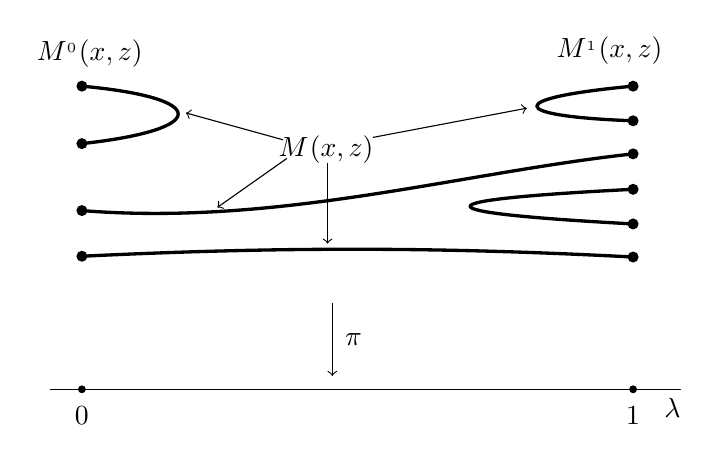
\begin{tikzpicture}[line cap=round,line join=round]
\fill (0,4.40) circle (0.07);
\fill (0,3.67) circle (0.07);
\fill (0,2.82) circle (0.07);
\fill (0,2.24) circle (0.07);
\fill (7,4.40) circle (0.07);
\fill (7,3.96) circle (0.07);
\fill (7,3.54) circle (0.07);
\fill (7,3.09) circle (0.07);
\fill (7,2.65) circle (0.07);
\fill (7,2.23) circle (0.07);
\node[above] at (0.1,4.52) {$\scr{M}^{\varGamma_{0}}(x,z)$};
\node[above] at (6.7,4.55) {$\scr{M}^{\varGamma_{1}}(x,z)$};
\draw[very thick] (0,4.40) .. controls (1.63,4.25) and (1.63,3.85) .. (0,3.67);
\draw[very thick] (7,4.40) .. controls (5.37,4.25) and (5.37,4.02) .. (7,3.96);
\draw[very thick] (7,3.09) .. controls (4.24,2.95) and (4.24,2.80) .. (7,2.65);
\draw[very thick] (0,2.82) .. controls (2.5,2.62) and (4.8,3.30) .. (7,3.54);
\draw[very thick] (0,2.24) .. controls (2.5,2.36) and (4.5,2.36) .. (7,2.23);
\node at (3.10,3.60) {$\scr{M}^{\varGamma}(x,z)$};
\draw[->] (2.55,3.72) -- (1.32,4.06);
\draw[->] (3.70,3.75) -- (5.65,4.12);
\draw[->] (2.60,3.48) -- (1.72,2.86);
\draw[->] (3.12,3.42) -- (3.12,2.40);
\draw[->] (3.18,1.64) -- (3.18,0.72);
\node at (3.45,1.18) {$\pi$};
\draw (-0.4,0.55) -- (7.6,0.55);
\fill (0,0.55) circle (0.05);
\fill (7,0.55) circle (0.05);
\node[below] at (0,0.45) {$0$};
\node[below] at (7,0.45) {$1$};
\node at (7.5,0.32) {$\lambda$};
\end{tikzpicture}
\caption{}
\label{fig:gamma-cobordism}
\end{figure}

\begin{figure}[htbp]
\centering
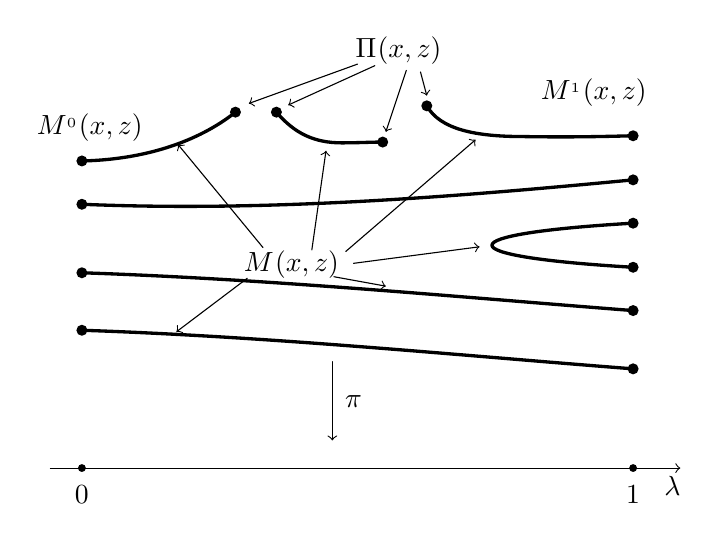
\begin{tikzpicture}[line cap=round,line join=round]
\fill (0,4.45) circle (0.07);
\fill (0,3.90) circle (0.07);
\fill (0,3.03) circle (0.07);
\fill (0,2.30) circle (0.07);
\fill (7,4.77) circle (0.07);
\fill (7,4.21) circle (0.07);
\fill (7,3.66) circle (0.07);
\fill (7,3.10) circle (0.07);
\fill (7,2.55) circle (0.07);
\fill (7,1.81) circle (0.07);
\node[above] at (0.1,4.57) {$\scr{M}^{\varGamma_{0}}(x,z)$};
\node[above] at (6.5,5.02) {$\scr{M}^{\varGamma_{1}}(x,z)$};
\fill (1.95,5.07) circle (0.07);
\fill (2.47,5.07) circle (0.07);
\fill (3.82,4.69) circle (0.07);
\fill (4.38,5.15) circle (0.07);
\draw[very thick] (0,4.45) .. controls (0.90,4.47) and (1.55,4.75) .. (1.95,5.07);
\draw[very thick] (2.47,5.07) .. controls (2.70,4.80) and (2.95,4.68) .. (3.30,4.68)
  .. controls (3.50,4.68) and (3.68,4.69) .. (3.82,4.69);
\draw[very thick] (4.38,5.15) .. controls (4.55,4.85) and (5.00,4.76) .. (5.60,4.76)
  .. controls (6.20,4.75) and (6.60,4.76) .. (7,4.77);
\node at (4.02,5.85) {$\Pi^{\varGamma}(x,z)$};
\draw[->] (3.50,5.68) -- (2.12,5.18);
\draw[->] (3.72,5.66) -- (2.62,5.16);
\draw[->] (4.12,5.60) -- (3.86,4.82);
\draw[->] (4.30,5.58) -- (4.38,5.28);
\draw[very thick] (0,3.90) .. controls (2.4,3.80) and (4.8,4.00) .. (7,4.21);
\draw[very thick] (7,3.66) .. controls (4.61,3.52) and (4.61,3.24) .. (7,3.10);
\draw[very thick] (0,3.03) .. controls (2.4,2.95) and (4.8,2.72) .. (7,2.55);
\draw[very thick] (0,2.30) .. controls (2.4,2.22) and (4.8,1.98) .. (7,1.81);
\node at (2.66,3.13) {$\scr{M}^{\varGamma}(x,z)$};
\draw[->] (2.30,3.35) -- (1.22,4.66);
\draw[->] (2.92,3.32) -- (3.10,4.58);
\draw[->] (3.35,3.30) -- (5.00,4.72);
\draw[->] (3.45,3.15) -- (5.05,3.36);
\draw[->] (3.20,2.98) -- (3.86,2.86);
\draw[->] (2.10,2.96) -- (1.20,2.28);
\draw[->] (3.18,1.90) -- (3.18,0.90);
\node at (3.45,1.40) {$\pi$};
\draw[->] (-0.4,0.55) -- (7.6,0.55);
\fill (0,0.55) circle (0.05);
\fill (7,0.55) circle (0.05);
\node[below] at (0,0.45) {$0$};
\node[below] at (7,0.45) {$1$};
\node at (7.5,0.32) {$\lambda$};
\end{tikzpicture}
\caption{}
\label{fig:gamma-cobordism-parity}
\end{figure}

\subsection{\trGluing}
\label{subsec:the-gluing}

当 $\mu(x)=\mu(z)$ 时，$\Pi^{\varGamma}(x,z)$ 的一个点就是一条破碎\trTrajectory，它可以是：
\begin{itemize}
\item 形如 $[\widehat{u}',(\lambda',v')]\in\scr{L}_{(H^{a},J^{a})}(x,y')\times\scr{M}^{\varGamma}(y',z)$ 的点；或者
\item 形如 $[(\lambda,u),\widehat{v}]\in\scr{M}^{\varGamma}(x,y)\times\scr{L}_{(H^{b},J^{b})}(y,z)$ 的点，
\end{itemize}
其中 $y'\in\operatorname{Crit}(\scr{A}_{H^{a}})$ 满足 $\mu(x)-\mu(y')=1$，或者 $y\in\operatorname{Crit}(\scr{A}_{H^{b}})$ 满足 $\mu(y)-\mu(z)=1$。

为了结束\cref{thm:compact-one-dimensional}部分（ii）的证明，我们使用一个类似于\cref{subsec:gluing-gamma}中那个过程的\trGluing{}过程，来对 $\Pi^{\varGamma}(x,z)$ 的每个点构造一个（于 $\scr{M}^{\varGamma}(x,z)$ 中的）\trEmbedding{} $\rho\mapsto\psi(\rho)$，这将给出\trManifoldWithBoundary{} $\scr{M}^{\varGamma}(x,z)\cup\Pi^{\varGamma}(x,z)$ 在所论的 $\Pi^{\varGamma}(x,z)$ 的那个点附近的一个\trParametrization。

我们将只限于对形如 $[(\lambda,u),\widehat{v}]$ 的点来做这件事，因为对其余各点的证明是类似的。精确的陈述如下。

\begin{theorem}\label{thm:gluing-near-broken}
设 $x$ 是 $\scr{A}_{H^{a}}$ 的一个\trCriticalPoint，并设 $y$、$z$ 是 $\scr{A}_{H^{b}}$ 的两个\trCriticalPoint，使得
\[
\mu(x)=\mu(z)=\mu(y)-1\text{。}
\]
设 $(\lambda_{\star},u)\in\scr{M}^{\varGamma}(x,y)$，并设 $\widehat{v}\in\scr{L}_{(H^{b},J^{b})}(y,z)$。那么：
\begin{itemize}
\item 存在一个\trEmbedding{} $\psi\colon[\rho_{0},+\infty[\,\to\scr{M}^{\varGamma}(x,z)$（对某个 $\rho_{0}$），使得 $\lim_{\rho\to+\infty}\psi(\rho)=[(\lambda_{\star},u),\widehat{v}]$；
\item 如果 $[\lambda_{n},\ell_{n}]$ 是 $\scr{M}^{\varGamma}(x,z)$ 的元素所成的一个趋于 $[(\lambda_{\star},u),\widehat{v}]$ 的序列，那么对充分大的 $n$，有 $[\lambda_{n},\ell_{n}]\in\operatorname{Im}\psi$。
\end{itemize}
\end{theorem}

这条定理中的\trConvergence{}就是\cref{thm:convergence-broken-gamma}中所定义的那一个。其证明将在下一节中给出。
